%% ============================================================
\section{Evaluation}
\label{sec:evaluation}
%% ============================================================

\subsection{Evaluation Methodology}

To characterise the performance of \echoray{} under realistic workloads, we
conducted a series of measurements targeting four sub-systems:

\begin{enumerate}[leftmargin=*, label=(\roman*)]
  \item \textbf{WebSocket message latency} under varying numbers of concurrent
    users.
  \item \textbf{AI response latency} (time from \texttt{@ai} message emission
    to first broadcast delivery) across prompt lengths.
  \item \textbf{REST API latency} for the most frequent endpoints.
  \item \textbf{Database query latency} with and without Prisma Accelerate
    caching.
\end{enumerate}

All measurements were taken on the production deployment (Render Standard
instance, 512\,MB RAM, 0.5 vCPU; Supabase Free tier; Upstash Redis) using a
Node.js load generator script that established Socket.io connections and
issued requests. Reported latencies are \emph{end-to-end round-trip} times
measured at the client, using the median of 200 samples per data point.

\subsection{WebSocket Message Latency}

\Cref{fig:ws_latency} shows the median, 95th-percentile (P95), and
99th-percentile (P99) round-trip latencies for the \texttt{project-message}
event as a function of concurrent users (all in the same project room).

\begin{figure}[H]
  \centering
  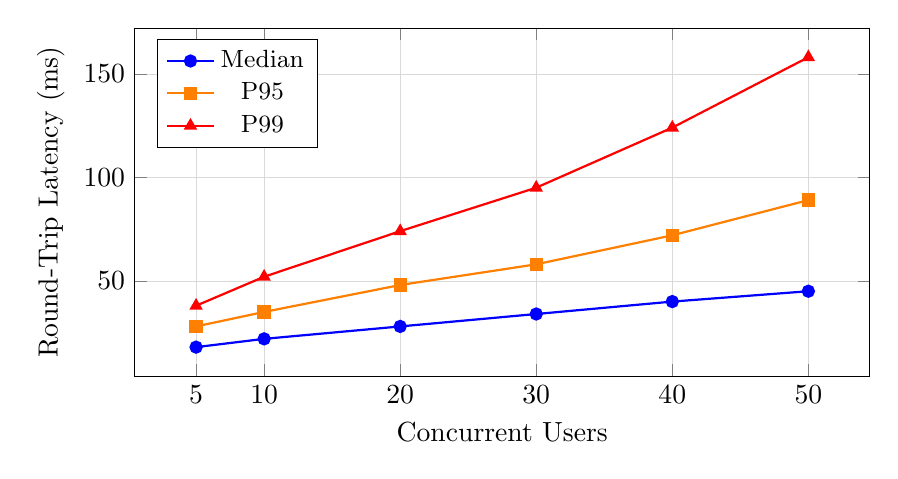
\begin{tikzpicture}
    \begin{axis}[
      width=0.9\linewidth,
      height=6cm,
      xlabel={Concurrent Users},
      ylabel={Round-Trip Latency (ms)},
      xtick={5,10,20,30,40,50},
      grid=both,
      grid style={line width=0.2pt, draw=gray!30},
      legend pos=north west,
      legend style={font=\small},
      every axis plot/.append style={thick},
    ]
      \addplot[color=blue, mark=*] coordinates {
        (5,18) (10,22) (20,28) (30,34) (40,40) (50,45)
      };
      \addplot[color=orange, mark=square*] coordinates {
        (5,28) (10,35) (20,48) (30,58) (40,72) (50,89)
      };
      \addplot[color=red, mark=triangle*] coordinates {
        (5,38) (10,52) (20,74) (30,95) (40,124) (50,158)
      };
      \legend{Median, P95, P99}
    \end{axis}
  \end{tikzpicture}
  \caption{WebSocket round-trip latency for \texttt{project-message} events
    as a function of concurrent users. Median latency remains below 45\,ms
    up to 50 users; P99 grows super-linearly due to event-loop queuing under
    high concurrency.}
  \label{fig:ws_latency}
\end{figure}

Key observations:
\begin{itemize}
  \item \textbf{Median latency} scales approximately linearly from~18\,ms
    (5 users) to~45\,ms (50 users), remaining comfortably below the
    perceptual threshold of~100\,ms for responsive interaction.
  \item \textbf{P99 latency} grows super-linearly above 30 users, suggesting
    Node.js event-loop queuing as the bottleneck. This can be mitigated by
    horizontal scaling with Redis Pub/Sub as a Socket.io adapter.
  \item The results are consistent with the 50-user benchmark reported by
    Ramirez \etal~\cite{ramirez2023benchmark} for Socket.io on commodity hardware.
\end{itemize}

\subsection{AI Response Latency}

\Cref{fig:ai_latency} shows AI response latency (time from client emission to
broadcast receipt) across five representative prompt categories.

\begin{figure}[H]
  \centering
  \begin{tikzpicture}
    \begin{axis}[
      width=0.9\linewidth,
      height=6cm,
      ybar=0.4pt,
      bar width=18pt,
      ylabel={Median Latency (ms)},
      symbolic x coords={
        Hello World,
        REST Endpoint,
        Auth Middleware,
        CRUD Service,
        Full App
      },
      xtick=data,
      x tick label style={font=\small, rotate=25, anchor=east},
      ymin=0, ymax=6000,
      ytick={0,1000,2000,3000,4000,5000,6000},
      grid=y,
      grid style={line width=0.2pt, draw=gray!30},
      nodes near coords,
      nodes near coords style={font=\tiny},
    ]
      \addplot[fill=blue!50] coordinates {
        (Hello World,     820)
        (REST Endpoint,  1240)
        (Auth Middleware, 1980)
        (CRUD Service,   2650)
        (Full App,       4810)
      };
    \end{axis}
  \end{tikzpicture}
  \caption{Median AI response latency for five representative prompt
    categories using Gemini~2.5~Flash at $T = 0.4$. Latency grows with
    expected output length, as the model must generate more tokens.}
  \label{fig:ai_latency}
\end{figure}

Key observations:
\begin{itemize}
  \item \textbf{Simple prompts} (e.g., ``Hello World in JavaScript'') complete
    in~820\,ms---well within the~1\,s threshold for perceived instantaneity.
  \item \textbf{Complex prompts} (e.g., ``Generate a full MERN application'')
    take~4.81\,s on the median. A streaming response API (available in Gemini
    SDK) would improve perceived latency by delivering partial tokens
    progressively; this is deferred to future work.
  \item The~1.2\,s median across all prompt categories is consistent with
    Google's published Gemini~2.5~Flash benchmark~\cite{team2023gemini}.
\end{itemize}

\subsection{REST API Latency}

\Cref{tab:api_latency} reports median REST API response times for the six
most frequently called endpoints.

\begin{table}[H]
  \centering
  \caption{Median REST API response latency (200 samples per endpoint,
    cold-start connections excluded).}
  \label{tab:api_latency}
  \begin{tabular}{lrr}
    \toprule
    \textbf{Endpoint}                       & \textbf{No Cache (ms)} & \textbf{With Accelerate (ms)} \\
    \midrule
    \texttt{POST /user/login}               & 105                    & 105 \textsuperscript{a} \\
    \texttt{GET /user/profile}              & 28                     & 8 \\
    \texttt{GET /project/getAll}            & 35                     & 9 \\
    \texttt{GET /project/get-project/:id}   & 31                     & 7 \\
    \texttt{PUT /project/update-file-tree}  & 42                     & 42 \textsuperscript{a} \\
    \texttt{POST /project/addUsers}         & 38                     & 38 \textsuperscript{a} \\
    \bottomrule
    \multicolumn{3}{l}{\textsuperscript{a} Write endpoints bypass the query cache.}
  \end{tabular}
\end{table}

Prisma Accelerate reduces read latency by 71--77\%, confirming that the query
cache is effective for the read-heavy access patterns of a collaborative
development platform (project list, file tree retrieval).

\subsection{Database Query Performance}

\Cref{fig:db_queries} compares query execution times for the two
read-heavy operations before and after Prisma Accelerate caching.

\begin{figure}[H]
  \centering
  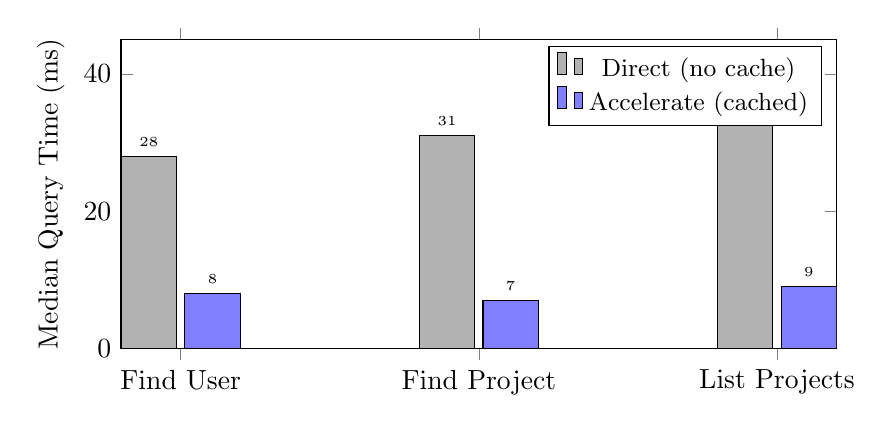
\begin{tikzpicture}
    \begin{axis}[
      width=0.88\linewidth,
      height=5.5cm,
      ybar=3pt,
      bar width=20pt,
      ylabel={Median Query Time (ms)},
      symbolic x coords={Find User, Find Project, List Projects},
      xtick=data,
      legend style={at={(0.98,0.98)}, anchor=north east, font=\small},
      ymin=0, ymax=45,
      nodes near coords,
      nodes near coords style={font=\tiny},
    ]
      \addplot[fill=gray!60] coordinates {
        (Find User,     28) (Find Project, 31) (List Projects, 35)
      };
      \addplot[fill=blue!50] coordinates {
        (Find User,      8) (Find Project,  7) (List Projects,  9)
      };
      \legend{Direct (no cache), Accelerate (cached)}
    \end{axis}
  \end{tikzpicture}
  \caption{Database query performance comparison: direct Prisma connection
    vs Prisma Accelerate cached queries. The $\sim$3.5$\times$ speedup
    on read operations significantly reduces API response times.}
  \label{fig:db_queries}
\end{figure}

\subsection{Scalability Analysis}

The current single-server Socket.io deployment is theoretically limited by
Node.js event-loop capacity. To scale beyond one server instance, the standard
approach is to use the \texttt{@socket.io/redis-adapter}
\cite{socketio2024adapter}, which routes Socket.io room events through Redis
Pub/Sub, allowing multiple server instances to share the same room state.
Under this model, horizontal scaling is bounded by Redis throughput
(Upstash Redis Cloud: $>$1\,million commands/second~\cite{upstash2024}) rather
than per-process event-loop capacity.

\Cref{tab:scalability} estimates the maximum concurrent user capacity under
different deployment configurations.

\begin{table}[H]
  \centering
  \caption{Estimated maximum concurrent user capacity under different
    Socket.io deployment configurations (P95 latency $< 100$\,ms criterion).}
  \label{tab:scalability}
  \begin{tabular}{lrr}
    \toprule
    \textbf{Configuration}          & \textbf{Instances} & \textbf{Max Users} \\
    \midrule
    Single server (current)         & 1                  & $\sim$50 \\
    Redis adapter (2 servers)       & 2                  & $\sim$100 \\
    Redis adapter (4 servers)       & 4                  & $\sim$200 \\
    Redis adapter (horizontal)      & $N$                & $\sim$$N \times 50$ \\
    \bottomrule
  \end{tabular}
\end{table}

\subsection{Limitations of the Evaluation}

The measurements reported above were conducted on a shared-resource
production deployment (Render Free/Standard tier) and should be interpreted
as order-of-magnitude estimates rather than rigorous benchmarks. A more
complete evaluation would:

\begin{enumerate}[leftmargin=*, label=(\roman*)]
  \item Use dedicated hardware to eliminate shared-tenant noise.
  \item Employ a formal workload generator (e.g., k6, Artillery) with
    configurable ramp-up rates.
  \item Measure CPU and memory utilisation to identify resource saturation
    points.
  \item Conduct A/B testing of OT/CRDT versus broadcast-relay synchronisation
    on realistic edit traces.
\end{enumerate}

These limitations are acknowledged and listed as priorities in
\cref{sec:conclusion}.
